\section{Evaluation}
\label{res_overview}

\begin{table*}[h]
    \centering
    \caption{Evaluation results overview. We evaluate two versions of mbed TLS and five
        versions of OpenSSL\@. CF represents secret-dependent control-flow transfers and
        DF represents secret-dependent data-flow transfers. A summary of all vulnerabilities 
        with the amount of leaked information can be found in the appendix.
    }\label{table:over_result}
    \newlength{\x}
    \newlength{\y}
    \settowidth{\x}{~~}
    \settowidth{\y}{m}
    \addtolength{\x}{-1\y}
    \newcommand{\foo}{\mbox{\hspace*{\the\x}}}
    \resizebox{2\columnwidth}{!}{

    \begin{tabular}{clrrrrrrr}
        \hline
        \textbf{Algorithm} & \textbf{Implementation}  & \textbf{Leakage Sites} & \textbf{CF}         & \textbf{DF}
                           & \textbf{\# Instructions} & \textbf{Max Leakage}   & \textbf{Sym.\ Exe.} & \textbf{Monte Carlo}                                                    \\\hline
                           &                          &                        &                     &                      &             & bits & ms        & ms              \\\cline{7-9}
        AES                & Mbed TLS 2.5             & 68                     & 0                   & 68                   & 39,855      & 8.6  & 512 ~~    & 1,052 ~~        \\
        AES                & Mbed TLS 2.15            & 68                     & 0                   & 68                   & 39,855      & 9.1  & 520 ~~    & 1,057 ~~        \\
        AES                & OpenSSL 0.9.7            & 75                     & 0                   & 75                   & 1,704       & 10.6 & 231 ~~    & 9,199 ~~        \\
        AES                & OpenSSL 1.0.2f           & 88                     & 0                   & 88                   & 1,350       & 12.0 & 36 ~~     & 1,924 ~~        \\
        AES                & OpenSSL 1.0.2k           & 88                     & 0                   & 88                   & 1,350       & 12.5 & 35 ~~     & 1,961 ~~        \\
        AES                & OpenSSL 1.1.0f           & 88                     & 0                   & 88                   & 1,420       & 12.6 & 36 ~~     & 2,161 ~~        \\
        AES                & OpenSSL 1.1.1            & 88                     & 0                   & 88                   & 1,586       & 4.4  & 43 ~~     & 1,631 ~~        \\
        DES                & Mbed TLS 2.5             & 15                     & 0                   & 15                   & 4,596       & 1.1  & 58 ~~     & 162 ~~          \\
        DES                & Mbed TLS 2.15            & 15                     & 0                   & 15                   & 4,596       & 1.0  & 57 ~~     & 162 ~~          \\
        DES                & OpenSSL 0.9.7            & 6                      & 0                   & 6                    & 2,976       & 7.6  & 163 ~~    & 4,677       ~~  \\
        DES                & OpenSSL 1.0.2f           & 8                      & 0                   & 8                    & 2,593       & 9.8  & 166 ~~    & 6,509       ~~  \\
        DES                & OpenSSL 1.0.2k           & 8                      & 0                   & 8                    & 2,593       & 10.1 & 165 ~~    & 5,975        ~~ \\
        DES                & OpenSSL 1.1.0f           & 8                      & 0                   & 8                    & 4,260       & 8.8  & 182 ~~    & 5,292        ~~ \\
        DES                & OpenSSL 1.1.1            & 6                      & 0                   & 6                    & 8,272       & 7.5  & 229 ~~    & 5,152       ~~  \\
                           &                          &                        &                     &                      &             &      & minutes   & minutes         \\\cline{8-9}
        RSA                & Mbed TLS 2.5             & 6                      & 6                   & 0                    & 22,109,246  & 9.6  & 39 ~~     & 41  ~~          \\
        RSA                & Mbed TLS 2.15            & 12                     & 12                  & 0                    & 24,484,441  & 8.7  & 44 ~~     & 251  ~~         \\
        RSA                & OpenSSL 0.9.7            & 107                    & 105                 & 2                    & 17,002,523  & 17.2 & 23 ~~     & 428 ~~          \\
        RSA                & OpenSSL 1.0.2f           & 38                     & 27                  & 11                   & 14,468,307  & 16.2 & 29 ~~     & 436  ~~         \\
        RSA                & OpenSSL 1.0.2k           & 36                     & 27                  & 9                    & 15,285,210  & 14.2 & 40 ~~     & 714   ~~        \\
        RSA                & OpenSSL 1.1.0f           & 31                     & 22                  & 9                    & 16,390,750  & 17.2 & 34 ~~     & 490 ~~          \\
        RSA                & OpenSSL 1.1.1            & 27                     & 20                  & 7                    & 18,207,020  & 14.9 & 7 ~~      & 501 ~~          \\\hline
        Total              &                          & 886                    & 219                 & 667                  & 128,061,910 &      & 209m \foo & 2,861m \foo     \\\hline
        %                    &                          &                       &                     &                      &             & bits & ms        & ms              \\\cline{7-9}
        % AES                & Mbed TLS 2.5             & 68                    & 0                   & 68                   & 39,855      & 8    & 570 ~~    & 850 ~~          \\
        % AES                & Mbed TLS 2.15            & 68                    & 0                   & 68                   & 39,855      & 8    & 550 ~~    & 829 ~~          \\
        % AES                & OpenSSL 0.9.7            & 75                    & 0                   & 75                   & 1,704       & 10   & 319 ~~    & 7,720 ~~        \\
        % AES                & OpenSSL 1.0.2f           & 88                    & 0                   & 88                   & 1,350       & 12   & 72 ~~     & 1,500 ~~        \\
        % AES                & OpenSSL 1.0.2k           & 88                    & 0                   & 88                   & 1,350       & 11   & 83 ~~     & 1,441 ~~        \\
        % AES                & OpenSSL 1.1.0f           & 88                    & 0                   & 88                   & 1,420       & 12   & 87 ~~     & 1,454 ~~        \\
        % AES                & OpenSSL 1.1.1            & 88                    & 0                   & 88                   & 1,586       & 8    & 91 ~~     & 1,250 ~~        \\
        % DES                & Mbed TLS 2.5             & 15                    & 0                   & 15                   & 4,596       & 1    & 114 ~~    & 144 ~~          \\
        % DES                & Mbed TLS 2.15            & 15                    & 0                   & 15                   & 4,596       & 1    & 106 ~~    & 137 ~~          \\
        % DES                & OpenSSL 0.9.7            & 6                     & 0                   & 6                    & 2,976       & 7    & 149 ~~    & 4,193       ~~  \\
        % DES                & OpenSSL 1.0.2f           & 8                     & 0                   & 8                    & 2,593       & 9    & 239 ~~    & 5,311       ~~  \\
        % DES                & OpenSSL 1.0.2k           & 8                     & 0                   & 8                    & 2,593       & 9    & 235 ~~    & 5,080        ~~ \\
        % DES                & OpenSSL 1.1.0f           & 8                     & 0                   & 8                    & 4,260       & 9    & 256 ~~    & 5,027        ~~ \\
        % DES                & OpenSSL 1.1.1            & 6                     & 0                   & 6                    & 8,272       & 7    & 235 ~~    & 4,584       ~~  \\
        %                    &                          &                       &                     &                      &             &      & minutes   & minutes         \\\cline{8-9}
        % RSA                & Mbed TLS 2.5             & 6                     & 6                   & 0                    & 22,109,246  & 9    & 38 ~~     & 20  ~~          \\
        % RSA                & Mbed TLS 2.15            & 12                    & 0                   & 12                   & 24,484,441  & 9    & 39 ~~     & 241  ~~         \\
        % RSA                & OpenSSL 0.9.7            & 105                   & 103                 & 2                    & 16,980,109  & 13   & 28 ~~     & 266 ~~          \\
        % RSA                & OpenSSL 1.0.2f           & 38                    & 27                  & 11                   & 14,468,307  & 10   & 28 ~~     & 160  ~~         \\
        % RSA                & OpenSSL 1.0.2k           & 36                    & 27                  & 9                    & 15,285,210  & 12   & 39 ~~     & 282   ~~        \\
        % RSA                & OpenSSL 1.1.0f           & 31                    & 22                  & 9                    & 16,390,750  & 13   & 32 ~~     & 262 ~~          \\
        % RSA                & OpenSSL 1.1.1            & 26                    & 20                  & 6                    & 18,207,020  & 12   & 7 ~~      & 455 ~~          \\\hline
        % Total              &                          & 883                   & 205                 & 678                  & 128,042,089 &      & 213m \foo & 1,688m \foo     \\\hline
    \end{tabular}
    }
\end{table*}

We evaluate \tool{} on real-world crypto libraries, OpenSSL and mbed TLS\@. OpenSSL
is the most commonly used crypto libraries in today's software. mbed TLS\@
(previous known as PolarSSL) is designed to be easy to understand and fit on
small embedded devices.

We build the source code into 32-bit x86 Linux executables with the GCC 8.0
under Ubuntu 14.04. Although we use use symbol information to track back leakage
sites in the source code, our tool can also work on stripped binaries. We
develop a Pin tool based on Intel Pin (version 3.7) to record the execution
trace. We run our experiments on a 2.90GHz Intel Xeon(R) E5-2690 CPU with 128GB
RAM memory. During our evaluation process, we are interested in the following
aspects:
\begin{enumerate}
    \item  \textbf{Identifying side-channels leakages.}
          The first step of \tool{} is to identify side-channel leakages. Is
          \tool{} effective to detect side-channels in real-world crypto
          systems? (\S\ref{sec:eval_overview} and \S\ref{eval:scala})
    \item  \textbf{Quantifying side-channel leakages.}
          Can \tool{} precisely report the number of leaked bits in crypto
          libraries? Are the numbers of leaked bits reported by \tool{} useful
          to justify the severity levels of the side-channel vulnerabilities?
          (\S\ref{sec:eval_case}, \S\ref{sec::eval_rsa}, and \S\ref{sec:eval_countermeasures})
\end{enumerate}

\subsection{Evaluation Result Overview} \label{sec:eval_overview}
Table~\ref{table:over_result} shows the overview of evaluation results. \tool{} found
883 leakages in total from real-world crypto system libraries. Among those 883
leak points, 205 of them are leaked due to secret-dependent control-flow
transfers and 678 of them are leaked due to secret-dependent memory accesses.

\tool{} finds that secret-dependent memory accesses
cause most leakages. \tool{} also identifies that most side-channel
vulnerabilities leak very little information in practice, which confirms our
initial assumptions.  Without our tool, developers will not be able to
distinguish those ``vulnerabilities'' from severe ones and ignore them for sure.
However, we do find some vulnerabilities that \tool\ reports with more severe
leakages. Some of them have been confirmed by existing research that those
vulnerabilities can be exploited to realize real attacks.

All the symmetric encryption implementations in OpenSSL and mbed TLS\@ have significant
leakages due to the implementation of the lookup table to speed up the
computation. Every leakage found during the evaluation belongs to the type of
secret-dependent memory accesses. We believe that the secret-dependent
control-flow transfers have been widely studied in the past few years, and
developers have patched most of those leakages. 

\tool{} finds several leakage sites for both implementations of DES and AES in
OpenSSL and mbed TLS\@. \tool{} confirms that all those leakages come from table
lookups. mbed TLS 2.15 and 2.5 have the same implementations of DES and AES so
they have the same leakage report. One proper fix would be a scalar bit-sliced
implementation. However, we do not see the bit-sliced implementation of AES and
DES in various versions of OpenSSL and mbed TLS\@. However, we find the new
implementation of OpenSSL instead uses typical four 1K tables. It only uses one 1K
of the tables. This implementation is rather easy but is still vulnerable to a
side channel attack. However, the countermeasures do somehow decrease the total
amount of leaked information as the quantification result shown in the next
section.

We also evaluates our tool on the RSA implementation. With the optimization
introduced in \S\ref{sec:scala}, we do not apply any domain knowledge to
simplify the analysis. Therefore, our tools can not only identify all the leakage sites
reported by CacheD~\cite{203878}, but find new leakages in a shorter time. 
We also find the newer
versions of RSA in OpenSSL tend to have fewer leakages detected by \tool{}. We
will discuss the version changes and corresponding leakages in the next section.

\tool{} can also estimate how
much information is leaked from each vulnerability. \tool{} achieves the goal by
estimating number of keys that satisfy the constraints. During the evaluation,
for each leakage site, \tool{} will stop once 1) it has 95\% confidence
possibility that the error of estimated leaked information is less than 1 bit,
which gives us confidence on the leakage quantification with the \emph{precision guarantee}, 
or 2) it cannot reach the termination condition after 10 minutes. In
the latter case, it means the number of satisfying keys is very small and the
leakage is quite severe. \emph{That is, timeout indicates severe leakage.}
%The tool marks the Monte Carlo is failed.
%\label{loc:timeout}
%During the evaluation,
%we find \tool{} can quantify every side-channel leakage for every symmetric
%encryption. For asymmetric encryptions, Monte Carlo sometimes
%times out. 
We manually check those leakage sites and find most of them are quite severe.
We will present the details in the subsequent sections.

\subsection{Comparison with the Existing Tools}
%\subsection{Scalability}
\label{eval:scala}

%% Fix tonight
%\subsubsection{Running Time}
%\begin{figure}
%    \centering
%    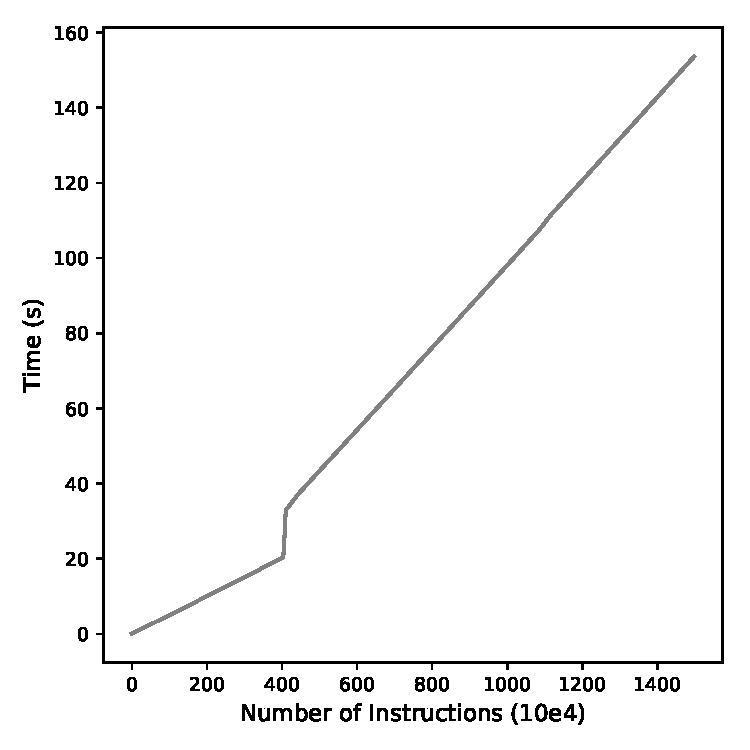
\includegraphics[width=.8\columnwidth]{./figures/result/running_time.pdf}
%    \caption{With the optimization introduced, \tool{} can be scalable to RSA}
%\end{figure}

%\subsubsection{Comparison with the Existing Tools}
\tool{} is designed to quantify side-channel leakages. But it can detect
side-channels leakages as well. In this section, we compare \tool{} with the
existing trace-based side-channel identification tools.

As shown in Table~\ref{eval:cacheD},
\tool{} can not only identify all the leakage sites reported by CacheD~\cite{203878}, but also
many new ones. CacheD fails to detect many vulnerabilities for two
reasons. First, CacheD can only detect secret-dependent memory access
vulnerabilities. But \tool{} can detect secret-dependent control-flows as well.
Second, CacheD suffers from some performance issues and uses some domain
knowledge to simplify symbolic execution and has to trim the traces before
processing. The design does not introduce false positives, but can neglect some
vulnerabilities. On the contrary, \tool{} does not apply any domain knowledge
and can find more vulnerabilities. The table~\ref{eval:cacheD} shows that
\tool{} is three times faster than CacheD. As the time of symbolic execution
grow quadratically, \tool{} is much faster than CacheD when analyzing the same
number of instructions. For example, when we test~\tool{} on AES from OpenSSL
0.9.7, ~\tool{} is more than 100x faster than CacheD.

Since DATA~\cite{217537} compares several execution traces to identify
side-channel leakages, \tool{} also outperforms DATA in terms of performance.
For example, it takes 234 minutes for DATA to analysis the RSA of implementation
in OpenSSL 1.1.0f. \tool{} only spends 34 minutes according to Table~\ref{table:over_result}.
Also, DATA reports report 278 control-flow and 460 data leaks. Among those leakages,
they found two vulnerabilities. On the contrary, \tool{} can report how many bits is
actually leaked, which eases the pain to discover sensitive leakages.

\begin{table}[]
    \caption{Comparison with CacheD}
    \label{eval:cacheD}
    \resizebox{\columnwidth}{!}{%
        \begin{tabular}{c|c|c|c|ccc}
            \hline
            \multicolumn{1}{l|}{} & \multicolumn{2}{c|}{Number of Instructions} & \multicolumn{2}{c|}{Time (s)} & \multicolumn{2}{c}{Number of Leakages}                                                                                         \\ \cline{2-7}
            \multicolumn{1}{l|}{} & \multicolumn{1}{c|}{CacheD}                 & \multicolumn{1}{c|}{\tool}    & \multicolumn{1}{c|}{CacheD}            & \multicolumn{1}{c|}{\tool}  & \multicolumn{1}{c|}{CacheD} & \multicolumn{1}{c}{\tool} \\ \hline
            AES 0.9.7             & 791                                         & 1,704                         & 43.4                                   & \multicolumn{1}{c|}{0.30}   & \multicolumn{1}{c|}{48}     & 75                        \\
            AES 1.0.2f            & 2,410                                       & 1,350                         & 48.5                                   & \multicolumn{1}{c|}{0.08}   & \multicolumn{1}{c|}{32}     & 88                        \\
            RSA 0.9.7             & 674,797                                     & 16,980,109                    & 199.3                                  & \multicolumn{1}{c|}{1681}   & \multicolumn{1}{c|}{2}      & 105                       \\
            RSA 1.0.2f            & 473,392                                     & 14,468,307                    & 165.6                                  & \multicolumn{1}{c|}{1692}   & \multicolumn{1}{c|}{2}      & 38                        \\ \hline
            Total                 & 1,151,390                                   & 31,451,470                    & 456.8                                  & \multicolumn{1}{c|}{3373.4} & \multicolumn{1}{c|}{84}     & 317                       \\ \hline
            \multicolumn{7}{l}{\# of Instructions per second \qquad  CacheD: 2,519 \qquad \tool: 9,324}                                                                                                                                          \\ \hline
        \end{tabular}
    }
\end{table}

\subsection{Vulnerability Case Study}\label{sec:eval_case}
\subsubsection{AES in mbed TLS}
During our evaluation, we find mbed TLS 2.5 and 2.15.1 have the same
implementation of AES\@. Our tool provides the same leakage report for both
versions. \tool{} identifies that most leakages are in function
\emph{mbedtls\_internal\_aes\_decrypt}. (Other leakage sites are in function
\emph{mbedtls\_aes\_setkey\_enc}.) All leakages are caused by secret-dependent
memory accesses. Shown in Appendix~\ref{mbedtls_aes}, there are seven leakage
sites in total. Leakage 1, 2, 3 are the same and leakage 4, 5, 6, 7 are the
same. They both use a pre-computed lookup table to speed up computation.
However, \tool{} reports leakage 1, 2, 3 typically leak more information
compared to leakage 4, 5, 6, 7. We check the source code and find leakage 1, 2,
3 use secret to access the lookup table \emph{RT0, RT1, RT2, RT3}, which is 8K
each. On the contrary, leakage 4, 5, 6, 7 each accesses a smaller lookup table
(2K). Therefore, leakage 4, 5, 6, 7 leak less information.



\subsubsection{RSA in mbedTLS}
\tool{} identifies several side-channel leakages for the RSA implementation in
Mbed TLS. Here we introduce and analyze two cases.
%, as shown in Figure~\ref{fig:mbedtls_rsa_1} and \ref{fig:mbedtls_rsa_2}.

\tool{} reports one bit information is leaked from the branch at line 2 in
Figure~\ref{fig:mbedtls_rsa_1} and it leaks less information than other
leakages. Function \emph{mbedtls\_mpi\_exp\_mod} performs sliding-window
exponentiation for big numbers. The leakage is caused by checking the signed bit
of the big number $N$. Therefore, the leakage can only tell whether $N$ is
greater than zero, which is one bit leak, not severe.

\begin{figure}%[h!]
    \centering
    \begin{lstlisting}[xleftmargin=.02\textwidth,xrightmargin=.01\textwidth]
...
if( mbedtls_mpi_cmp_int( N, 0 ) < 0 || ( N->p[0] & 1 ) == 0 )
    return( MBEDTLS_ERR_MPI_BAD_INPUT_DATA );
...
\end{lstlisting}
    \vspace*{-6pt}
    \caption{Function \textit{mbedtls\_mpi\_exp\_mod}}
    \label{fig:mbedtls_rsa_1}
    \vspace*{-6pt}
\end{figure}

\begin{figure}%[h!]
    \centering
    \begin{lstlisting}[xleftmargin=.02\textwidth,xrightmargin=.01\textwidth]
...
do {
    *d += c; c = ( *d < c ); d++;
}
while( c != 0 );
...
\end{lstlisting}
    \vspace*{-6pt}
    \caption{Function \textit{mpi\_mul\_hlp}}
    \label{fig:mbedtls_rsa_2}
    \vspace*{-6pt}
\end{figure}

Function \emph{mpi\_mul\_hlp}, shown in Figure~\ref{fig:mbedtls_rsa_2},
is notoriously for a series of timing attacks.
Recent patches have fixed many leakages in function \emph{mpi\_mul\_hlp}.
\tool{} reports 8 bits of information is leaked from line 5.
\emph{mpi\_mul\_hlp} is a helper function to perform mbedtls\_mpi
multiplication. As the code will be executed many times, each time it will leak
independent information. The leakage is severe compared to the previous one.

\subsection{Case Study of RSA in OpenSSL} \label{sec::eval_rsa}
For the crypto libraries, it is likely that an updated version has less
vulnerabilities compared to the previous versions because software developers
have patched some of those vulnerabilities.

We test five versions of OpenSSL (0.9.7, 1.0.2f, 1.0.2k, 1.1.0f, 1.1.1). The
result, as shown in Figure~\ref{fig:rsa}, confirms our assumptions. The newer
version of OpenSSL leaked less amount of information compared to the previous
versions. After version 0.9.7g, OpenSSL adopted a fixed-window mod\_exp
implementation for RSA\@. With the new design, the sequence of squares and
multiples and the memory access patterns are independent of the secret key.
\tool{}'s result confirms the new exponentiation implementation has quite
effectively mitigated most of leakages because the other four versions have fewer
leakages than 0.9.7. OpenSSL version 1.0.2f, 1.0.2k and 1.1.0f almost have the
same amount of leakage. We check the changelog and find only one change for
patching vulnerabilities for RSA (CVE-2016-0702). RSA changelog also claims
OpenSSL 1.1.1 adopted ``numerous side-channel attack mitigation.'' The result
confirms our assumptions.

\begin{figure*}
    \centering
    \vspace*{-9pt}
    \hspace*{-8pt}
    \subfloat[RSA OpenSSL 0.9.7]{
        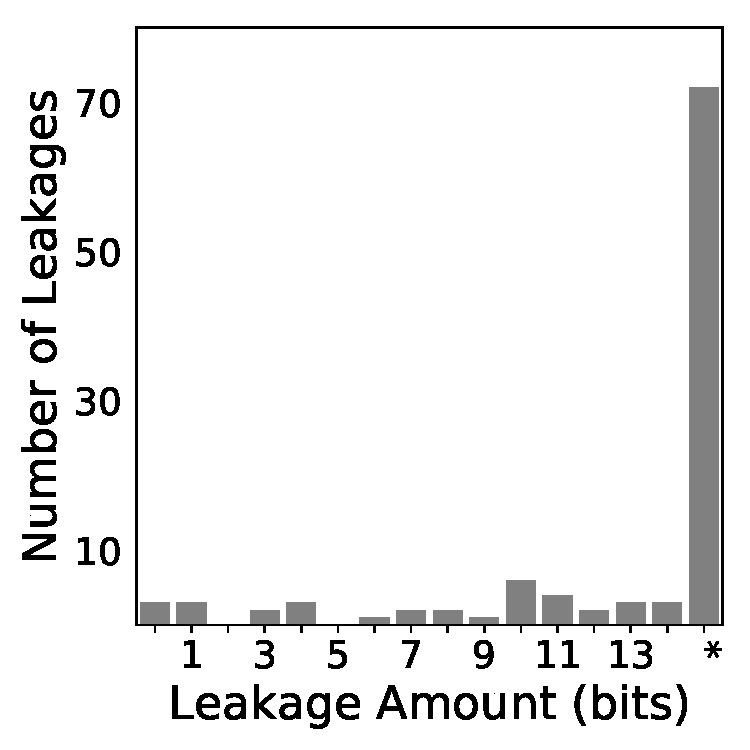
\includegraphics[width=.19\linewidth]{./figures/result/RSA-openssl-0-9-7.pdf}
        \label{fig:rsa-1}
    }
    \subfloat[RSA OpenSSL 1.0.2f]{
        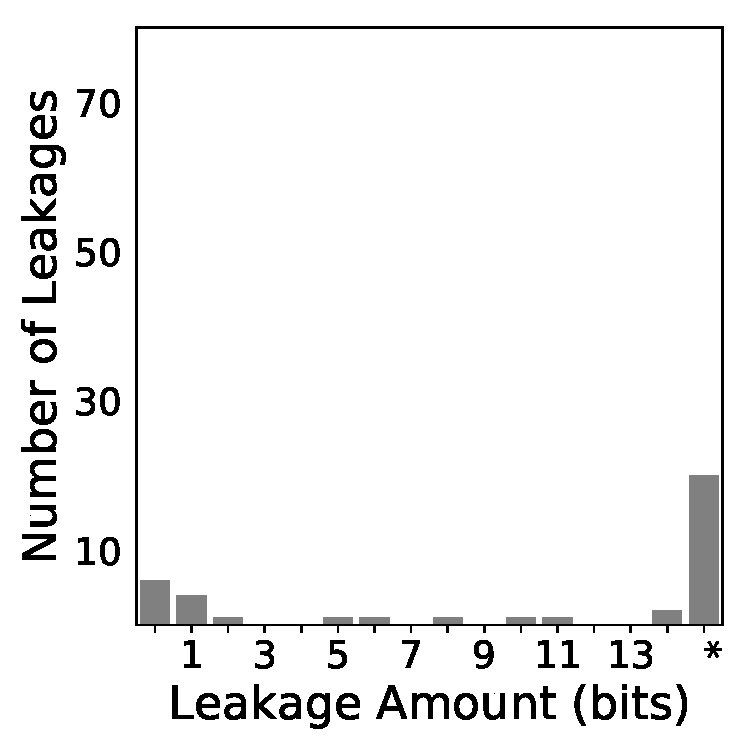
\includegraphics[width=.19\linewidth]{./figures/result/RSA-openssl-1-0-2f.pdf}
        \label{fig:rsa-2}
    }
    \subfloat[RSA OpenSSL 1.0.2k]{
        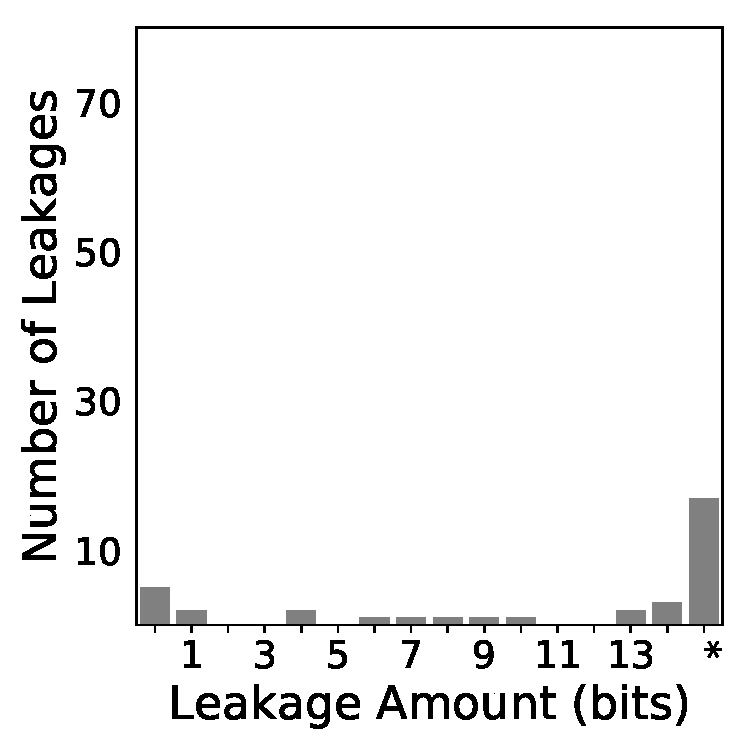
\includegraphics[width=.19\linewidth]{./figures/result/RSA-openssl-1-0-2k.pdf}
        \label{fig:rsa-3}
    }
    \subfloat[RSA OpenSSL 1.1.0f]{
        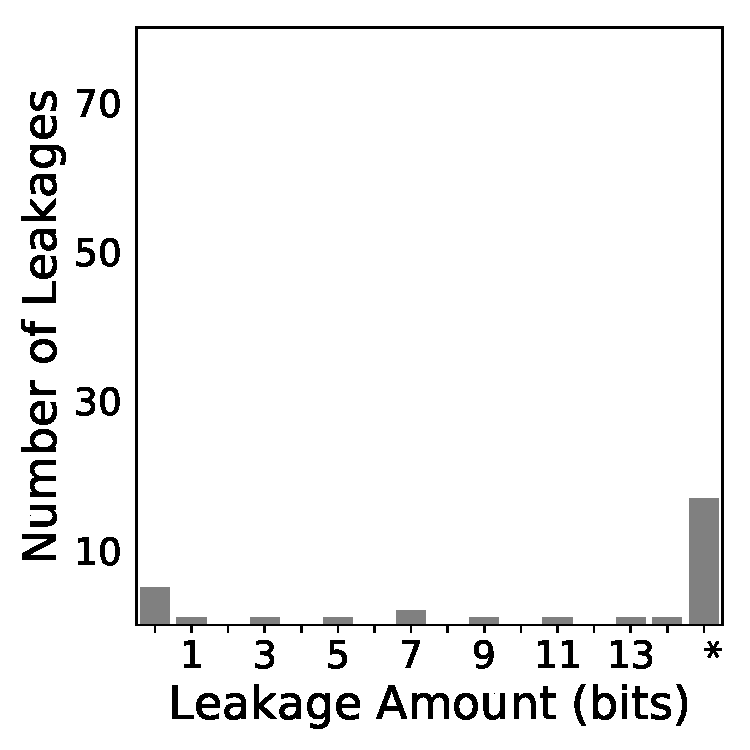
\includegraphics[width=.19\linewidth]{./figures/result/RSA-openssl-1-1-0f.pdf}
        \label{fig:rsa-4}
    }
    \subfloat[RSA OpenSSL 1.1.1]{
        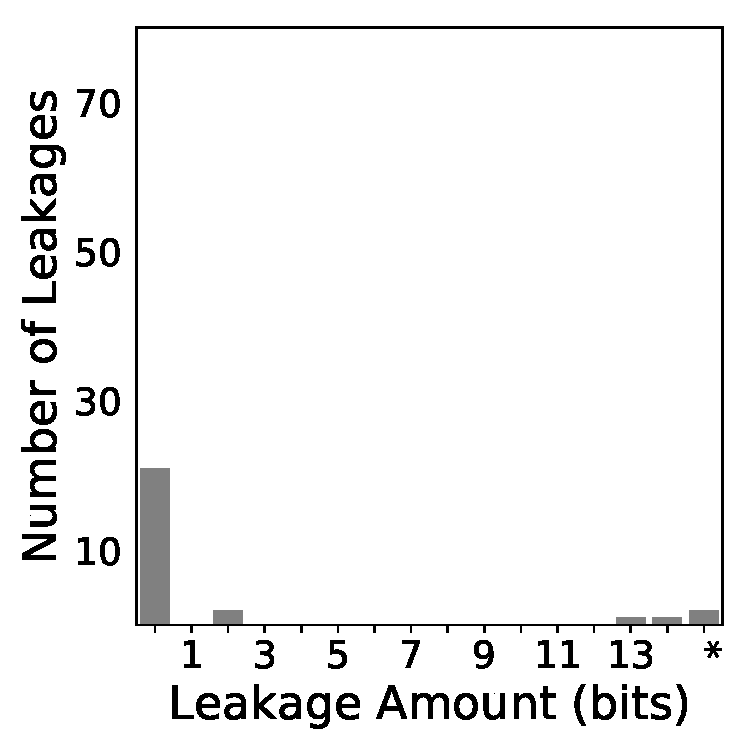
\includegraphics[width=.19\linewidth]{./figures/result/RSA-openssl-1-1-1.pdf}
        \label{fig:rsa-5}
    }
    \caption{RSA implementations in different versions of OpenSSL\@. 
        We round the number of leaked information into the nearest integer. 
        The mark $*$ means timeout,
        which indicates more severe leakages (see \S\ref{loc:timeout}).}
    \label{fig:rsa}
    \vspace*{-12pt}
\end{figure*}

\subsection{Analysis of Software Countermeasures}\label{sec:eval_countermeasures}
\subsubsection{Bit-slicing}

Bit-slicing is an efficient method to construct constant-time implementation for
side channel to mitigation. The basic concept is to
implement a function in terms of single-bit logical gate operations, such as AND, XOR, OR,
and NOT\@.
% Eli Biham et al.~\cite{Biham:1997:FND:647932.757246} first use gate
% circuits to implement the SBOX of DES\@. Based on his work Matthew
% Kwan~\cite{Kwan2000ReducingTG} present a better implementation of DES with fewer
% gates and first used the term Bit-slicing. 
% This approach can immune cryptographic algorithms to cache and timing-related
% side-channel attacks. 
%Figure~\ref{fig:SBOX_bitslicing} describe a Bit-slicing implement of
%secret-depend Substitution-box (SBOX) shown in Figure~\ref{fig:SBOX_da}.
Since the table lookups and conditional jumps are replaced with single-bit
logical gates, with no secret-dependent memory addresses or control flow, both
the data access and control flow types of side-channel leakages are mitigated.

We would like to test \tool\ on bit-slicing. We adopted the SBOX
implementations, commonly used in block ciphers such as DES and AES, with and
without bit-slicing, and apply \tool\ to confirm the mitigation. The SBOX
implementation with and without bit-slicing are shown in
Figure~\ref{fig:SBOX_bitslicing} and Figure~\ref{fig:SBOX_da}, respectively, in
Appendix~\ref{appendix:SBOX}. Consider an SBOX take some bits derived from a
password as input and output 2-bit transform result. The plain implementation
has a range check on the password input and a secret-dependent table lookup
while bit-slicing does not.
%% The plain implementation will first ensure the input does not overflow
%% and then directly access the table for the substitution result, as described in
%% Figure~\ref{fig:SBOX_da}. While we apply the Bit-sliding to this SBOX, the check
%% and access process will transfer to a series of logical operations described in
%% Figure~\ref{fig:SBOX_bitslicing}.
\tool\ reports that there are both control-flow and data access types of leakage
in the non-bit-slicing implementation
%% We apply \tool to both implementations.
%% According to the result, there exist two leakage sites in non-bit-slicing
%% implementation: one control-flow type leakage from check operation and one data
%% access type leakage from the table lookup operation of directly access method
(line 6 and line 7 in Figure~\ref{fig:SBOX_da}). The number of leaked bits is
5.0 and 4.4, respectively. At line 6, according to Definition~\ref{def}, the
input set $K$ is $[0,2^8-1]$, the observed input set $K^o$ is $[0,2^3-1]$. Thus,
the leakage $L_{\beta(k)\rightarrow o}$ based on the observation ($o$) is
$L_{\beta(k)\rightarrow o} = \log_2{|K|} - \log_2{|K^o|} = 8-3 = 5$ bit, which
confirms the result from \tool. Similarly, we can verify the result of the other
leakage site. \tool{} reports no leakage on the bit-slicing implementation.
% The basic concept is to express a function
% in terms of single-bit logical operations (AND, XOR, OR, NOT, etc.). These
% operations are then carried out for multiple instances of the function in
% parallel, using bitwise operations on a CPU. The original intention of
% Bit-slicing Implementation is to accelerate the crypto algorithms. However,
% thanks to the features of gate operations, the implementations gain additional
% security properties. Since the table lookup operation and conditional jump
% operation will be replaced with single-bit logical gates, without directly
% non-input data access or control flow change, thus both the data access type and
% control flow type of side-channel leakage will be avoided.

% \subsubsection{Scatter and Gather}
% The scatter-gather technology is also a common defence method to cache-based timing attacks.
% \begin{figure}[h!]
%     \centering
%     \begin{lstlisting}[xleftmargin=.02\textwidth,xrightmargin=.01\textwidth]
% ...
% align ( buf ):
%     return buf - ( buf & ( block size - 1 ) ) + block size

% scatter ( buf, p, k ):
%     for i := 0 to N - 1 do
%         buf [k + i * spacing] := p [k][i]

% gather ( r, buf, k ):
%     for i := 0 to N - 1 do
%         r [i] := buf [k + i * spacing]
% ...
% \end{lstlisting}
%     \caption{Scatter\_and\_Gather}
%     \label{Scatter_and_Gather}
% \end{figure}

% \begin{figure}[h!]
%     \centering
%     \begin{lstlisting}[xleftmargin=.02\textwidth,xrightmargin=.01\textwidth]
% ...
% uint8_t SBOX[] = {1, 0, 3, 1, 2, 2, 3, 0};
% align(buf);
% scatter(buf, SBOX, k);
% ...
% \end{lstlisting}
%     \caption{Sbox\_with\_Scatter\_and\_Gather}
%     \label{SBOX_sg}
% \end{figure}

\subsubsection{Smaller Lookup Tables}
Considering the cache-collision timing attack \cite{Bonneau11894063_16}, the
probability of leakage decreases when the lookup table entry or element size gets
smaller. We take AES as an example, for the last round of encryption, the algorithm
uses a specialized table with 4-byte size entries, of which only one
byte from each element actually contributes to the result. Hence, a significant method to reduce
the information leakage in AES is to reduce the size of the lookup table. We
designed a demo to illustrate this countermeasure, a lookup table with one-byte
size elements (see Figure~\ref{fig:one_byte_table}) will leak less information
than a table with 4-byte element size (see Figure~\ref{fig:four_byte_table}). 
The encrypt function for each table to process the same amount of information, 
respectively, (see Figure~\ref{fig:one_byte_table_lookup} and
Figure~\ref{fig:four_byte_table_lookup}).  \tool{} reports three leakage sites for
each lookup table, with 4.0 bits for the table with smaller entries and 2.0
bits for the table with bigger entries, confirming the theory.
